\chapter{Research Direction and Discussion}

This chapter presents the result of the literature study. It starts in Section~\ref*{sec:review} by presenting the review and analysis of the three \ac {RL} approaches explained in Chapter~\ref{chap::survey}. The review consists of parameters that are taken into considerations -- advantages, limitations and practical challenges for implementation. Section~\ref{sec:res_planning} presents the research plan which will be carried out during the thesis. In the end of the chapter, a discussion is covered in Section~\ref{sec:discussion}
\section{Review and Analysis of \ac{RL} Approaches} \label{sec:review}
\subsection{{\ac{RL} for Optimal Tracking Control}}
From the mathematical perspective, the optimal tracking approach is more rigorous compared to the other two. The proof of convergence, for instance, has been provided in literature \cite{1099755}. Another advantage is since the approach is based on lyapunov function, system's stability is guaranteed. Furthermore, researchers have successfully extended this approach to different control condition: discrete-continuous time, linear-nonlinear system, known-(partially)unknown model. From all of these benefits, the optimal tracking approach seems to be a suitable choice. However, there are some limitations which must be overcome in order to implement this method for a robotic tracking application.

As previously stated in the motivation, the goal of the thesis is to push the envelope of current tracking performance using \ac {RL}. As for the case-specific, it is hypothesized in Chapter~\ref{chap:testbed} that the low tracking performance is due to unknown non-linearities and disturbance in the robot. Therefore, a model-based standard optimal tracking is no longer a relevant solution. Although \cite{Kiumarsi20141167} has shown that using \ac{RL}, one can obviate the need of system model for linear system, the solution for an unknown non-linear system is not yet available. This is one crucial limitation to this method for now since we actually want to improve tracking of potentially non-linear system. Even if the solution exists, a practical problem will most probably arise due to the necessity of persistence of excitation in order to achieve a converging control policy \cite{Kiumarsi20141167} \cite{AlTamimi2007473}. For the UR5 robot testbed, this could potentially damage the robot since the motors must be excited with a persistently exciting signal such as pseudo-random noise. 

The second limitation of the approach is that it is still not known how to integrate the available but inaccurate model to the optimal tracking. Literatures have shown that although the models are not perfect, it can still help in speeding up the \ac {RL} convergence time \cite{Brujeni5669655} \cite{Grondman6096441}. Therefore, model integration would be a useful, though not necessary factor. Due to these factors, optimal tracking \ac {RL} is not the most suitable method for the thesis requirements.

\subsection{Dynamic Tuning via \ac{RL}}
\subsubsection{Direct Tuning of Nominal Controller}
The advantage of the direct tuning by \ac{RL} is its simple, intuitive scheme and rather direct implementation. However, direct tuning \ac{RL} only works with a standard state/output feedback controller such as \ac{PID}. State/output feedback controller is known for its nature which is always "late" since it has to wait for the error to appear and then compensate for it. Throughout the literature survey, author could not find a paper which integrates an \ac{RL}-based dynamic tuning with more sophisticated controller such as optimal tracking control or \ac {MPC}. Due to this bottleneck in performance, the direct-tuning is not the best choice to answer the research's goal.
\subsubsection{Gain scheduling for \ac{DMP}}
As previously explained in Chapter~\ref{chap::survey}, \ac{PI$^2$} learns the optimum trajectory to enable robotic manipulator passing through a certain intermediate point described by \ac{DMP}. In order to use \ac{PI$^2$} \ac{DMP} for reference tracking, one would need to extend the point of attractor $g$ into a full trajectory $g(k)$. The answer of this problem, assuming that the question itself is relevant, is not present at this time.

In order to provide an answer to above problem, a thorough understanding of the \ac{PI$^2$} algorithm and \ac {DMP} approach is needed. This is a particularly challenging problem since to derive the \ac{PI$^2$} itself involves a rather complex procedures such as stochastic optimal control which can easily be misunderstood if not treated carefully \cite{Buchli2010}. Due to the needs of extensive theoretical study, duration constraint of the thesis and the risk that this method is ultimately irrelevant, it is decided that \ac {PI$^2$} \ac{DMP} is not the most suitable solution.

\subsection{Nonlinear Input Compensation via \ac{RL}}
To the best of author's knowledge, there is no any literature yet which addresses the implementation of this method to a full reference tracking task. The only existing work is presented in \cite{Efe2014} which compensates an unknown gravity for a \ac {PD}-controlled 1-\ac {DoF} robot arm acting on a simple step command. Thus, this method, if successfully implemented, can be considered a novel solution. This algorithm is also modular in the sense that the compensator acts as an additive signal which does not influence the controller's output. This means the better the nominal controller performs, the smaller tracking errors needs to be compensated. Furthermore, the compensator also does not require any information about the system model to operate. 

The drawback of this method is the lack of mathematical formalization to prove the common control criterion: stability, convergence and robustness. From the practical point of view, some kind of mechanism must be introduced to ensure that the compensator signal is not too large since the nominal controller has already performed near optimally. Nevertheless, due to the model-free characteristic, this method is chosen to be the solution which will be developed and implemented for the rest of the thesis.

\section{Research Plan} \label{sec:res_planning}
The post-literature survey research plan is organized as follows. Before commissioning the implementation on the UR5, a simple simulation of a 1-\ac {DoF} manipulator will be programmed. The purpose of the simulation is to verify that the proposed method is actually working. If the \ac{RL}-based optimizer indeed works, the next step would be to further develop the controller for implementation on the UR5 robot. If the controller performs as expected, improvement will be carried out until the end of the thesis. Parallel to these steps, the thesis report will be written as well. The research plan is summarized in a flowchart as shown in Figure~\ref{fig:flowchart}.

\begin{figure}
\centering
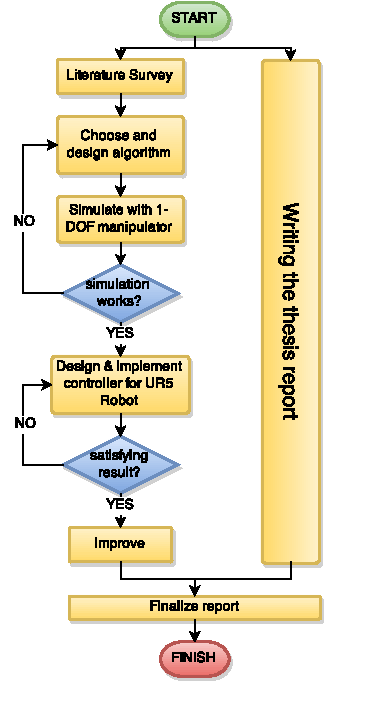
\includegraphics[width=0.5\linewidth]{research_plan.pdf}
\caption{Research plan flowchart}
\label{fig:flowchart}
\end{figure}

\section{Discussion}\label{sec:discussion}
Since Chapter~\ref{chap:testbed} has shown that for a simple straight line trajectory the jitter appears to be repetitive, author finds it interesting to compare \ac{RL} for reference tracking with a much more mature technique, namely \ac{ILC} \cite{4048052}. As the name suggested, \ac {ILC} is developed to improve tracking contaminated by repetitive error/disturbance. This method has been successfully implemented for various applications from CNC machining \cite{299157} to industrial robots \cite{1044377}. Therefore, \ac {ILC} could serve as a benchmark during later verification.
